
\documentclass[11pt]{article}
\usepackage[margin=0.85in]{geometry}
\usepackage{amsmath,amssymb}
\usepackage{booktabs}
\usepackage{graphicx}
\usepackage{hyperref}
\usepackage{float}
\usepackage{array}
\usepackage{longtable}
\usepackage{caption}
\hypersetup{colorlinks=true, linkcolor=blue, urlcolor=blue}

\title{Report for Adaptive Newton-Schulz for Muon}
\date{June 2026}

\begin{document}
\maketitle

\begin{abstract}
This report evaluates adaptive Newton--Schulz coefficients for the Muon optimizer
on deterministic one-dimensional regression problems. The benchmark suite uses
explicit target formulas, six optimizers including Adam and AdamW, and multiple
model initializations. Results are reported as raw final losses, per-problem
final-loss ratios to the best method, and mean loss curves with one-standard-
deviation bands. The main empirical signal is that FastNS and the current
adaptive variant often give faster early loss decay. On the more difficult or
rougher targets, however, final-loss advantages are mixed, so the current
adaptive controller should be viewed as a conservative baseline rather than an
optimized policy.
\end{abstract}

\section{Newton--Schulz Coefficients}

Muon normalizes matrix-valued momentum updates with a short Newton--Schulz (NS)
iteration. After Frobenius normalization $X_0=M/(\|M\|_F+\epsilon)$, the degree-5
matrix update is
\begin{equation}
    X_{k+1} = aX_k + \left(bX_kX_k^\top + c(X_kX_k^\top)^2\right)X_k.
\end{equation}
On singular values this corresponds to $f(x)=ax+bx^3+cx^5$. The coefficient
$a=f'(0)$ determines how strongly small singular values are amplified. Larger
$a$ can speed up optimization, but it also increases overshoot and spike risk.

\section{Algorithms}

This section separates the algorithmic choices from the empirical protocol. There
are three pieces: scalar coefficient search, dense table construction, and the
online adaptive controller used inside Muon.

\subsection{Scalar Five-Step Stability Test}

For a candidate triple $(a,b,c)$, define $f(x)=ax+bx^3+cx^5$. The scalar test is
not an asymptotic fixed-point test. It directly tests the same five iterations
used by the optimizer:
\begin{verbatim}
input: coefficients (a,b,c), grid X = logspace(-3, 0, n)
for x in X:
    z = x
    for k = 1,...,5:
        z = a*z + b*z^3 + c*z^5
        reject if |z| > 2 or z is not finite
    reject if z not in [0.5, 1.5]
accept (a,b,c)
\end{verbatim}
The lower grid endpoint $10^{-3}$ is a modeling choice: singular values much
smaller than this have tiny effect after Frobenius normalization, while forcing
all values down to zero into the band would rule out useful aggressive
coefficients. The final band $[0.5,1.5]$ follows the empirical Muon observation
that exact convergence to one is unnecessary; a moderate spread of singular
values can still produce effective update directions. The intermediate orbit
bound $2$ is a guard against false positives where $f^5(x)$ happens to re-enter
the band after an explosive excursion.

\subsection{Random Search and Dense Table Construction}

The search maximizes the useful small-singular-value slope $a=f'(0)$ subject to
the five-step test. The implementation is batched: arrays of candidate triples
are sampled and evaluated on the whole scalar grid at once. The table generator
then buckets accepted triples by rounded $a$.
\begin{verbatim}
input: target range a = 3.50, 3.51, ..., 3.89
sample many triples:
    a ~ Uniform(3.47, 3.92)
    b ~ Uniform(-7.5, 0)
    c ~ Uniform(0.5, 4.5)
keep triples passing the five-step stability test
for each rounded target a:
    keep the accepted triple with largest actual a in that bucket
for missing or marginal buckets:
    run a narrower targeted search and validate on a denser grid
output: validated entries for muon/coeff_table.py
\end{verbatim}
The high-$a$ table begins at $3.50$ because lower values do not satisfy the
strict lower band from $x=10^{-3}$ in only five iterations. Lower entries
$(1.50,2.00,2.50,3.00,3.44)$ remain in the table as conservative warm-up,
rollback, and comparison points, but the dense strict-band part is the high-$a$
region. The upper end is $3.89$ because coefficients above roughly $3.9$ become
hard to validate under the final-band and orbit-boundedness constraints.

The runtime table is prepared before experiments rather than created on the fly.
It is stored in the \texttt{muon} package's \texttt{coeff\_table.py} module.
That module exposes \texttt{MUON\_COEFF\_TABLE} and pre-indexed key/value tuples
built once at import time. Each \texttt{AdaptiveMuon} instance reuses those
in-memory tuples and performs a nearest-lower binary lookup for the current
target $a_t$. Thus benchmark runs load the table before training starts; they do
not run coefficient search, load a JSON table from disk, or sort the table inside
the optimizer step. The optimizer has $a_{\max}=4.0$, but nearest-lower lookup
means targets above the largest table key use the $3.89$ entry unless the table
is extended.

\subsection{Adaptive Muon Family Baseline}

The current default adaptive method is not the old loss-spike dense-table
controller. It is a one-parameter table-schedule baseline. Only the scalar target
$a$ is scheduled; the Newton--Schulz triple is always selected from the prepared
coefficient table by nearest-lower lookup:
\begin{equation}
    a(\lambda) = (1-\lambda)a_{\rm FastNS} + \lambda a_{\rm fallback},
    \qquad (a,b,c) = \mathrm{lookup}(a(\lambda)),
    \qquad \lambda\in[0,1].
\end{equation}
Here $a_{\rm FastNS}=3.87$ is the FastNS table key and
$a_{\rm fallback}=3.62$ is the searched fallback table key. The fallback triple
stored at that key is $(3.624985,-7.285039,4.444867)$.

The fallback endpoint was chosen by a reproducible scalar-map screen over the
prepared table. Candidate endpoint keys are ranked by lower endpoint overshoot,
orbit size, and lower-tail lift, subject to the condition that every table entry
visited by the resulting $a$-schedule remains inside the strict five-step band.
This keeps the adaptive baseline on the validated coefficient table instead of
creating off-table triples by interpolating $(a,b,c)$ directly.

The default benchmark does not set a fixed transition time. It infers $t_0$
from a conservative spike-frequency comparison. Let $L_t$ be the current
training loss and $m_t$ be an exponential moving average of recent losses. A
local spike is recorded when $L_t > \tau m_{t-1}$. The trigger compares two
adjacent windows of length $W$: it starts the transition only when the current
window contains at least $s_{\min}$ spikes and at least $r$ more spikes than
the previous window:
\begin{verbatim}
input: step t, spike window W=40, spike threshold tau=1.25,
       EMA beta=0.98, min spikes s_min=2,
       count margin r=1, transition length T=100
before trigger: a_t = 3.87
spike_t = 1 if loss_t > tau * ema_loss_{t-1}, else 0
prev = sum(spike_{t-2W+1 : t-W})
curr = sum(spike_{t-W+1 : t})
if curr >= s_min and curr - prev >= r:
    t0 = t
lambda_t = 0 before t0, else clip((t - t0)/T, 0, 1)
a_t = (1-lambda_t)*3.87 + lambda_t*3.62
(a,b,c) = nearest_lower_lookup(MUON_COEFF_TABLE, a_t)
apply five Newton--Schulz iterations in the Muon update
\end{verbatim}
This signal does not use absolute loss levels, loss progress, or a zero-loss
assumption. It only reacts when local instability is becoming more frequent. A
fixed transition start remains available as an ablation through the command-line
option \texttt{--adaptive-transition-start}.

\subsection{Parameter Selection}

Table~\ref{tab:algorithm-parameters} lists the most important algorithmic
parameters and the reason they were chosen. These are not claimed to be globally
optimal; they are conservative defaults that make the experiments reproducible
and keep the adaptive mechanism interpretable.

\begin{table}[H]
\centering
\small
\begin{tabular}{p{0.24\linewidth}p{0.20\linewidth}p{0.48\linewidth}}
\toprule
Parameter & Value & Rationale \\
\midrule
NS steps $K$ & $5$ & Matches the Muon implementation; optimizing an asymptotic limit would solve the wrong problem. \\
Scalar grid & $[10^{-3},1]$ log-spaced & Focuses on practically relevant singular values after Frobenius normalization. \\
Final band & $[0.5,1.5]$ & Allows useful approximate orthogonalization without demanding exact convergence to one. \\
Orbit bound & $2$ & Rejects coefficients that temporarily escape even if $f^5$ returns to the band. \\
Search ranges & $a\in[3.47,3.92]$, $b\in[-7.5,0]$, $c\in[0.5,4.5]$ & Concentrates sampling around the empirically useful aggressive frontier while preserving enough room for varied curvature. \\
Dense table spacing & $0.01$ in $a$ & Provides candidate fallback endpoints and keeps nearest-lower lookup reproducible. \\
Start target & $a=3.87$ & Selects the FastNS table entry and gives the early aggressive small-mode amplification that fixed FastNS often benefits from. \\
Fallback endpoint & $a=3.62$ table entry & Table-mined non-Jordan endpoint with lower scalar overshoot than FastNS and a strict-band-stable table path from FastNS. \\
Transition trigger & spike-frequency increase & Starts from FastNS until the current 40-step window has at least 2 relative loss spikes and a spike-count increase of at least 1 relative to the previous window. \\
Spike definition & $L_t > 1.25 m_{t-1}$ & Uses local EMA baseline $m_t$ with beta $0.98$; this avoids assuming the optimum loss is zero. \\
Transition length & $100$ steps & Moves gradually after the detected $t_0$ so the run samples intermediate table keys. \\
Endpoint ranking & scalar-map heuristic & Ranks prepared-table endpoint keys by table-path stability, lower overshoot, orbit size, and lower-tail lift; future work should replace this with training-dependent energy-weighted criteria. \\
Adam/AdamW learning rate & $10^{-3}$ & Standard untuned baseline; future work should include learning-rate sweeps. \\
\bottomrule
\end{tabular}
\caption{Algorithmic parameters used in coefficient search, endpoint selection, and the current adaptive schedule.}
\label{tab:algorithm-parameters}
\end{table}

The main design tradeoff is that the trigger is intentionally conservative. It
can miss cases where switching earlier would improve final loss, but it avoids
using loss progress or an assumed zero floor. The next adaptive version should
combine this spike-frequency safety signal with gradient-value distribution
statistics, so the controller can distinguish ordinary minibatch roughness from
coefficient-induced instability.

\section{Project Structure}

The folder is organized as a research project: \texttt{muon/} contains the
optimizer, prepared coefficient table, and offline coefficient search;
\texttt{benchmarks/} contains benchmark problems, optimizer factories,
plotting, and the runner; \texttt{results/} stores numeric outputs;
\texttt{figures/} stores generated plots; and \texttt{docs/} stores this
report.

\section{Experiments}

\subsection{Benchmark Problems}

All targets are deterministic formulas on $[-1,1]$.

\begin{longtable}{p{0.19\linewidth}p{0.43\linewidth}p{0.30\linewidth}}
\caption{Benchmark target formulas.}\label{tab:problems}\\
\toprule
Problem & Formula & Purpose \\
\midrule
\endfirsthead
\toprule
Problem & Formula & Purpose \\
\midrule
\endhead
low\_frequency & $\sin(2\pi x)+0.30\cos(6\pi x)$ & Smooth low-frequency trigonometric target. \\
medium\_fourier & $0.70\sin(4\pi x)+0.40\sin(10\pi x+0.30)+0.20\cos(18\pi x-0.20)$ & Moderate Fourier mixture with three frequencies. \\
high\_frequency & $0.55\sin(8\pi x)+0.35\sin(18\pi x+0.40)+0.25\cos(34\pi x-0.10)+0.15\sin(58\pi x)$ & Higher-frequency Fourier mixture with four modes. \\
chirp\_quadratic & $\sin(2\pi(2x+7x^2))+0.25\sin(34\pi x)$ & Frequency-increasing chirp plus a high-frequency perturbation. \\
gaussian\_bumps & $\sum_i A_i\exp(-(x-c_i)^2/(2\sigma_i^2))$ with fixed five-bump parameters & Fixed mixture of narrow Gaussian bumps. \\
runge\_rational & $1/(1+25x^2)+0.15\sin(12\pi x)$ & Runge-style rational peak with sinusoidal ripple. \\
cusp\_abs & $|x|-0.50+0.25\sin(8\pi x)$ & Nonsmooth absolute-value cusp with oscillatory ripple. \\
multiscale\_mix & $0.45\sin(2\pi x)+0.25\sin(14\pi x+0.20)+0.12\cos(46\pi x)+0.35g_{\rm bumps}(x)$ & Low, medium, and high-frequency Fourier components plus localized bumps. \\
\bottomrule
\end{longtable}

\begin{figure}[H]
\centering
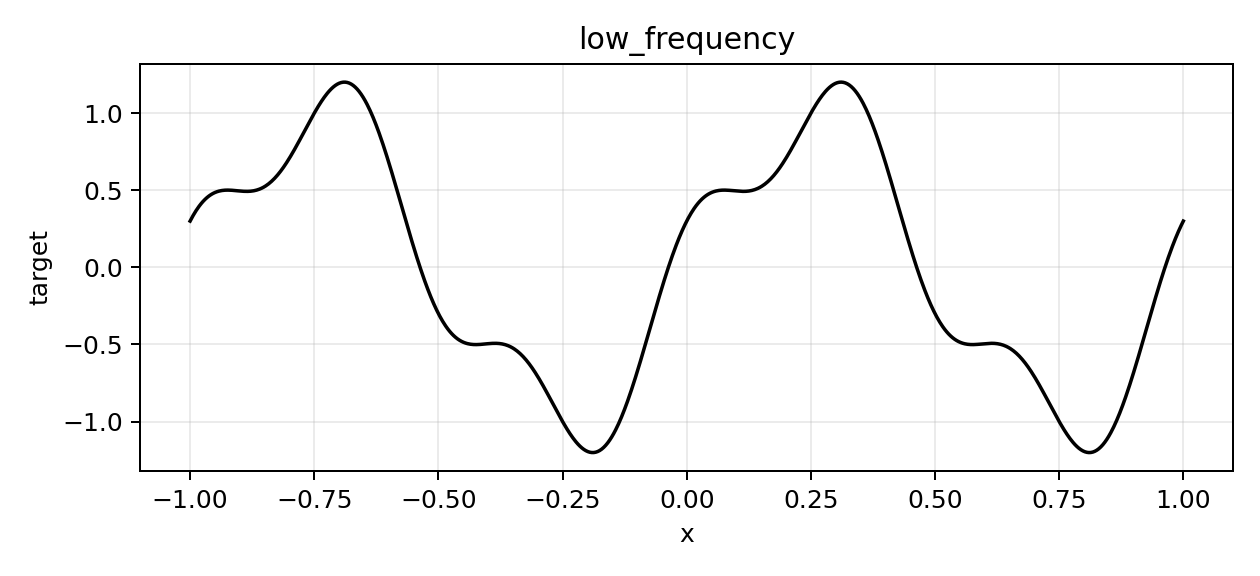
\includegraphics[width=0.47\linewidth]{../figures/adaptive_ns_suite/targets/low_frequency.png}
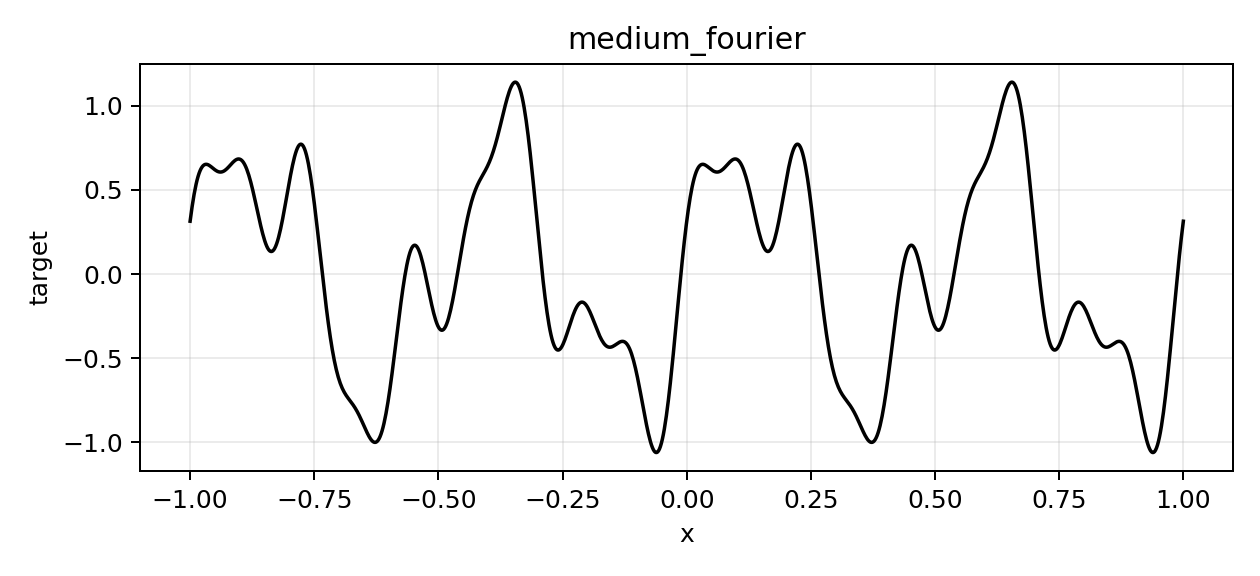
\includegraphics[width=0.47\linewidth]{../figures/adaptive_ns_suite/targets/medium_fourier.png}
\\
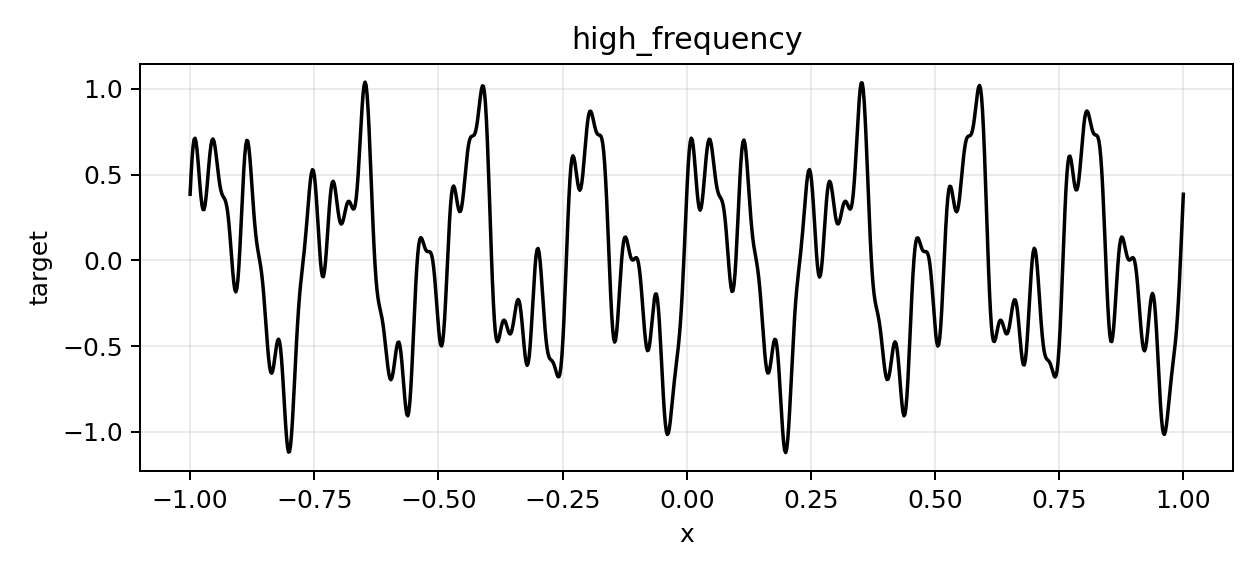
\includegraphics[width=0.47\linewidth]{../figures/adaptive_ns_suite/targets/high_frequency.png}
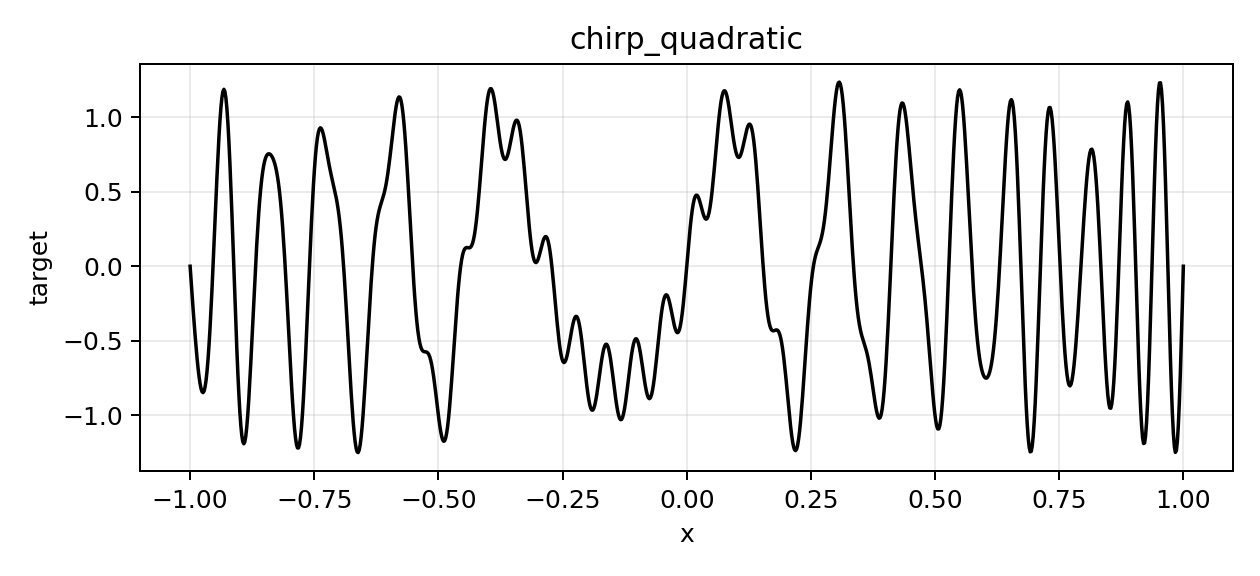
\includegraphics[width=0.47\linewidth]{../figures/adaptive_ns_suite/targets/chirp_quadratic.png}
\\
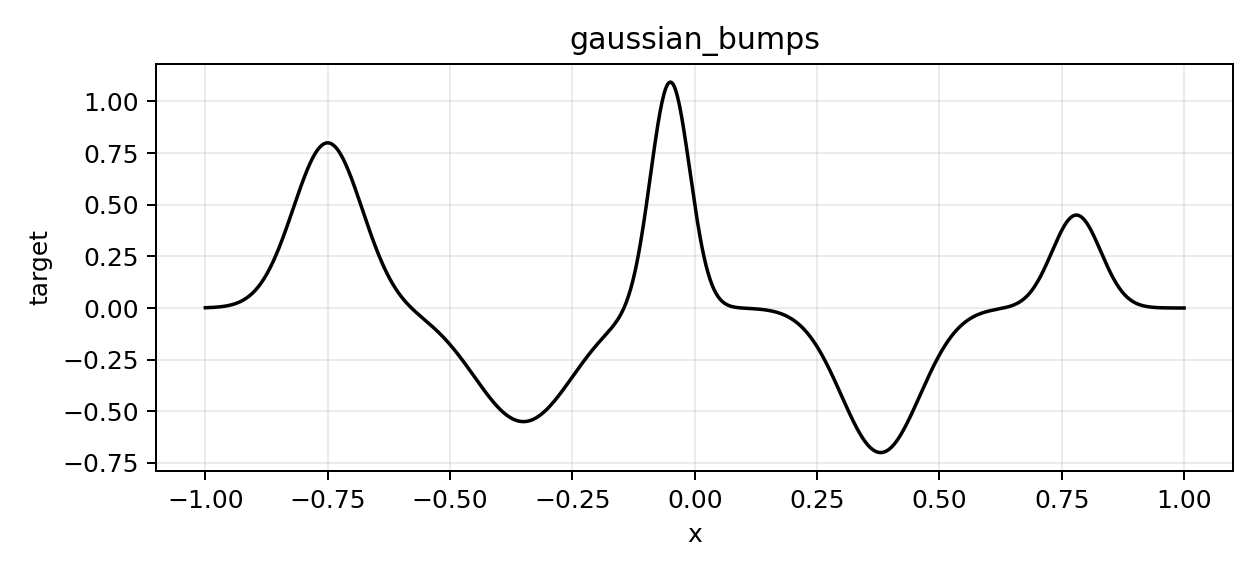
\includegraphics[width=0.47\linewidth]{../figures/adaptive_ns_suite/targets/gaussian_bumps.png}
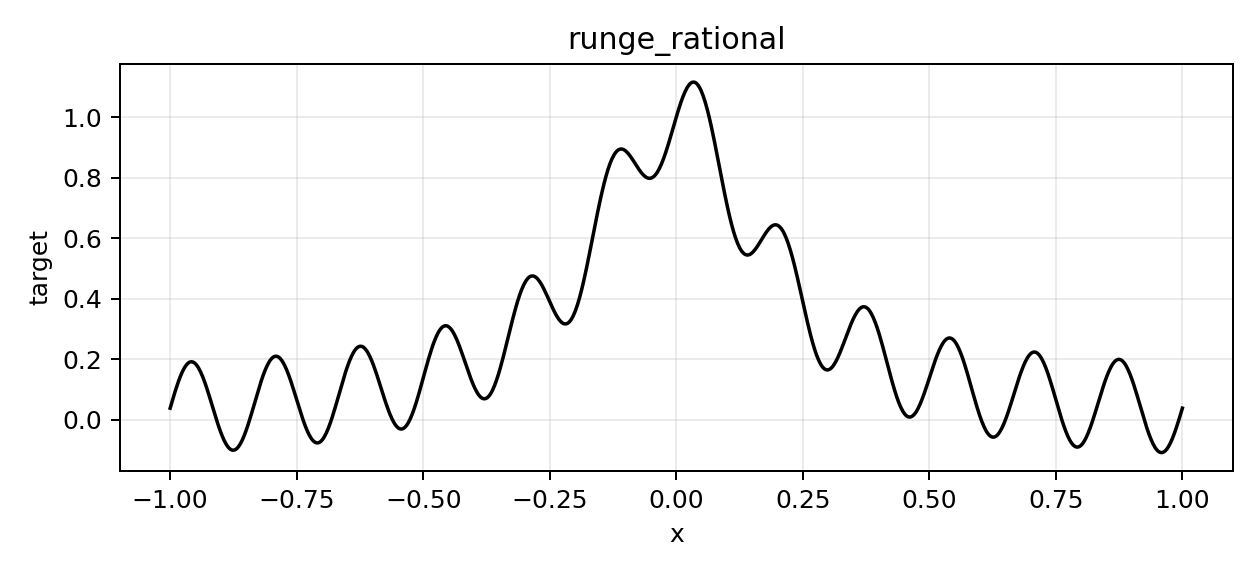
\includegraphics[width=0.47\linewidth]{../figures/adaptive_ns_suite/targets/runge_rational.png}
\\
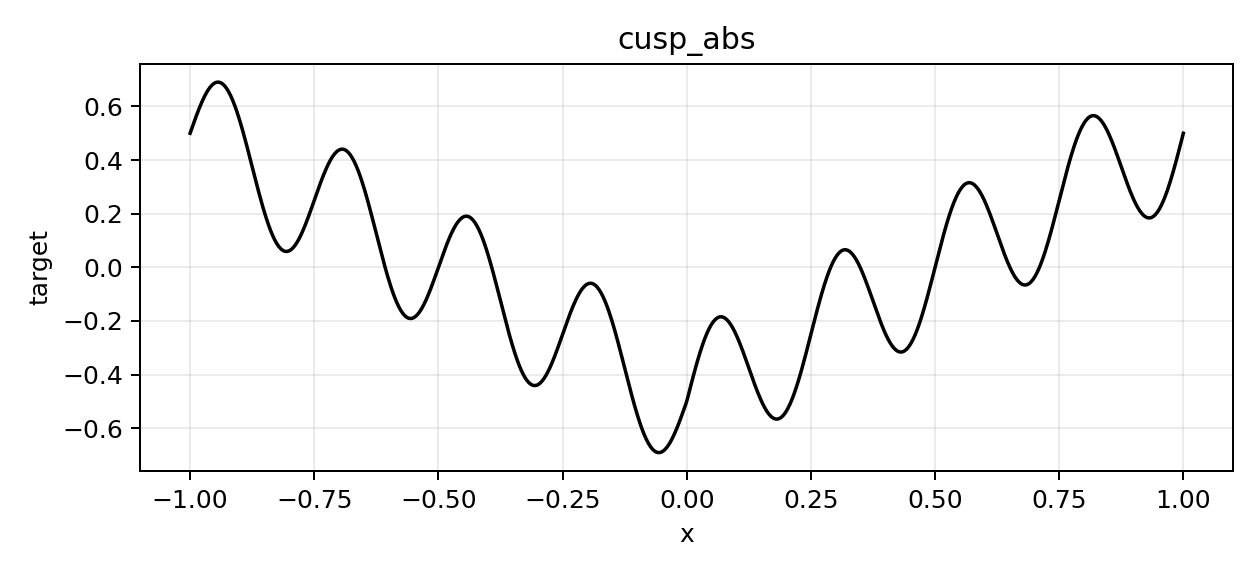
\includegraphics[width=0.47\linewidth]{../figures/adaptive_ns_suite/targets/cusp_abs.png}
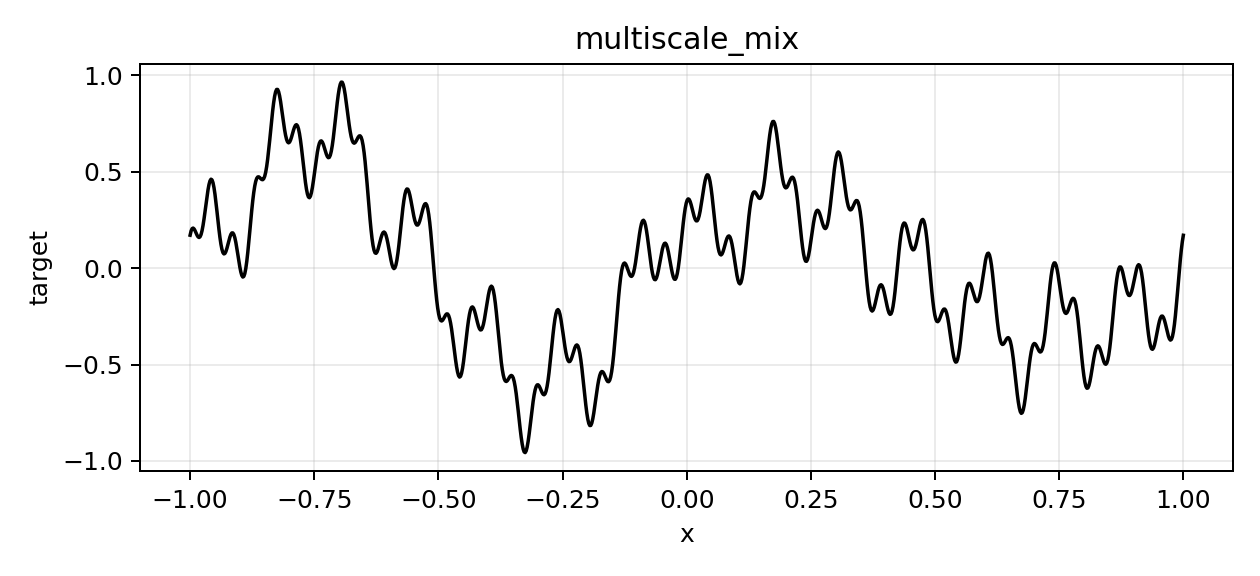
\includegraphics[width=0.47\linewidth]{../figures/adaptive_ns_suite/targets/multiscale_mix.png}
\\
\caption{Deterministic benchmark targets.}
\end{figure}

\subsection{Protocol}

Each method trains the same five-layer tanh MLP with hidden width $32$ for 500
epochs. Each problem/method pair is repeated over 20 initializations.
Training points are sampled uniformly from $[-1,1]$ with batch size 256. Adam uses
learning rate $10^{-3}$; AdamW uses learning rate $10^{-3}$ and weight decay
$10^{-2}$.

\subsection{Final Loss Ratios Per Problem}

Each table cell is \texttt{final MSE (ratio)}, where the ratio is relative to
the best final MSE on that problem. The best result in each row is boldfaced.

\begin{table}[H]
\centering
\scriptsize
\resizebox{\linewidth}{!}{%
\begin{tabular}{lrrrrrr}
\toprule
Problem & Standard & Jordan & FastNS & Adaptive & Adam & AdamW \\
\midrule
low\_frequency & 6.03e-02 (10.870) & 7.65e-03 (1.377) & 9.59e-03 (1.727) & \textbf{5.55e-03 (1.000)} & 6.11e-02 (11.005) & 6.12e-02 (11.028) \\
medium\_fourier & 2.12e-01 (4.584) & 5.51e-02 (1.191) & \textbf{4.62e-02 (1.000)} & \textbf{4.62e-02 (1.000)} & 2.99e-01 (6.474) & 2.99e-01 (6.475) \\
high\_frequency & 2.46e-01 (1.139) & \textbf{2.16e-01 (1.000)} & 2.20e-01 (1.019) & 2.20e-01 (1.019) & 2.48e-01 (1.146) & 2.48e-01 (1.146) \\
chirp\_quadratic & 5.03e-01 (1.174) & \textbf{4.28e-01 (1.000)} & 4.53e-01 (1.058) & 4.53e-01 (1.058) & 5.04e-01 (1.175) & 5.04e-01 (1.175) \\
gaussian\_bumps & 3.34e-02 (8.828) & 4.66e-03 (1.232) & 5.57e-03 (1.472) & \textbf{3.78e-03 (1.000)} & 1.27e-01 (33.683) & 1.28e-01 (33.734) \\
runge\_rational & 1.26e-02 (1.119) & 1.18e-02 (1.051) & 1.25e-02 (1.115) & 1.24e-02 (1.104) & \textbf{1.12e-02 (1.000)} & 1.12e-02 (1.000) \\
cusp\_abs & 3.24e-02 (1.065) & \textbf{3.04e-02 (1.000)} & 3.06e-02 (1.006) & 3.06e-02 (1.006) & 3.22e-02 (1.060) & 3.22e-02 (1.060) \\
multiscale\_mix & 4.34e-02 (1.184) & \textbf{3.67e-02 (1.000)} & 3.69e-02 (1.007) & 3.71e-02 (1.011) & 4.82e-02 (1.313) & 4.83e-02 (1.316) \\
\bottomrule
\end{tabular}
}
\caption{Mean final training MSE over 20 initializations, with per-problem final-loss ratio in parentheses.}
\label{tab:final-ratios}
\end{table}

\begin{figure}[H]
\centering
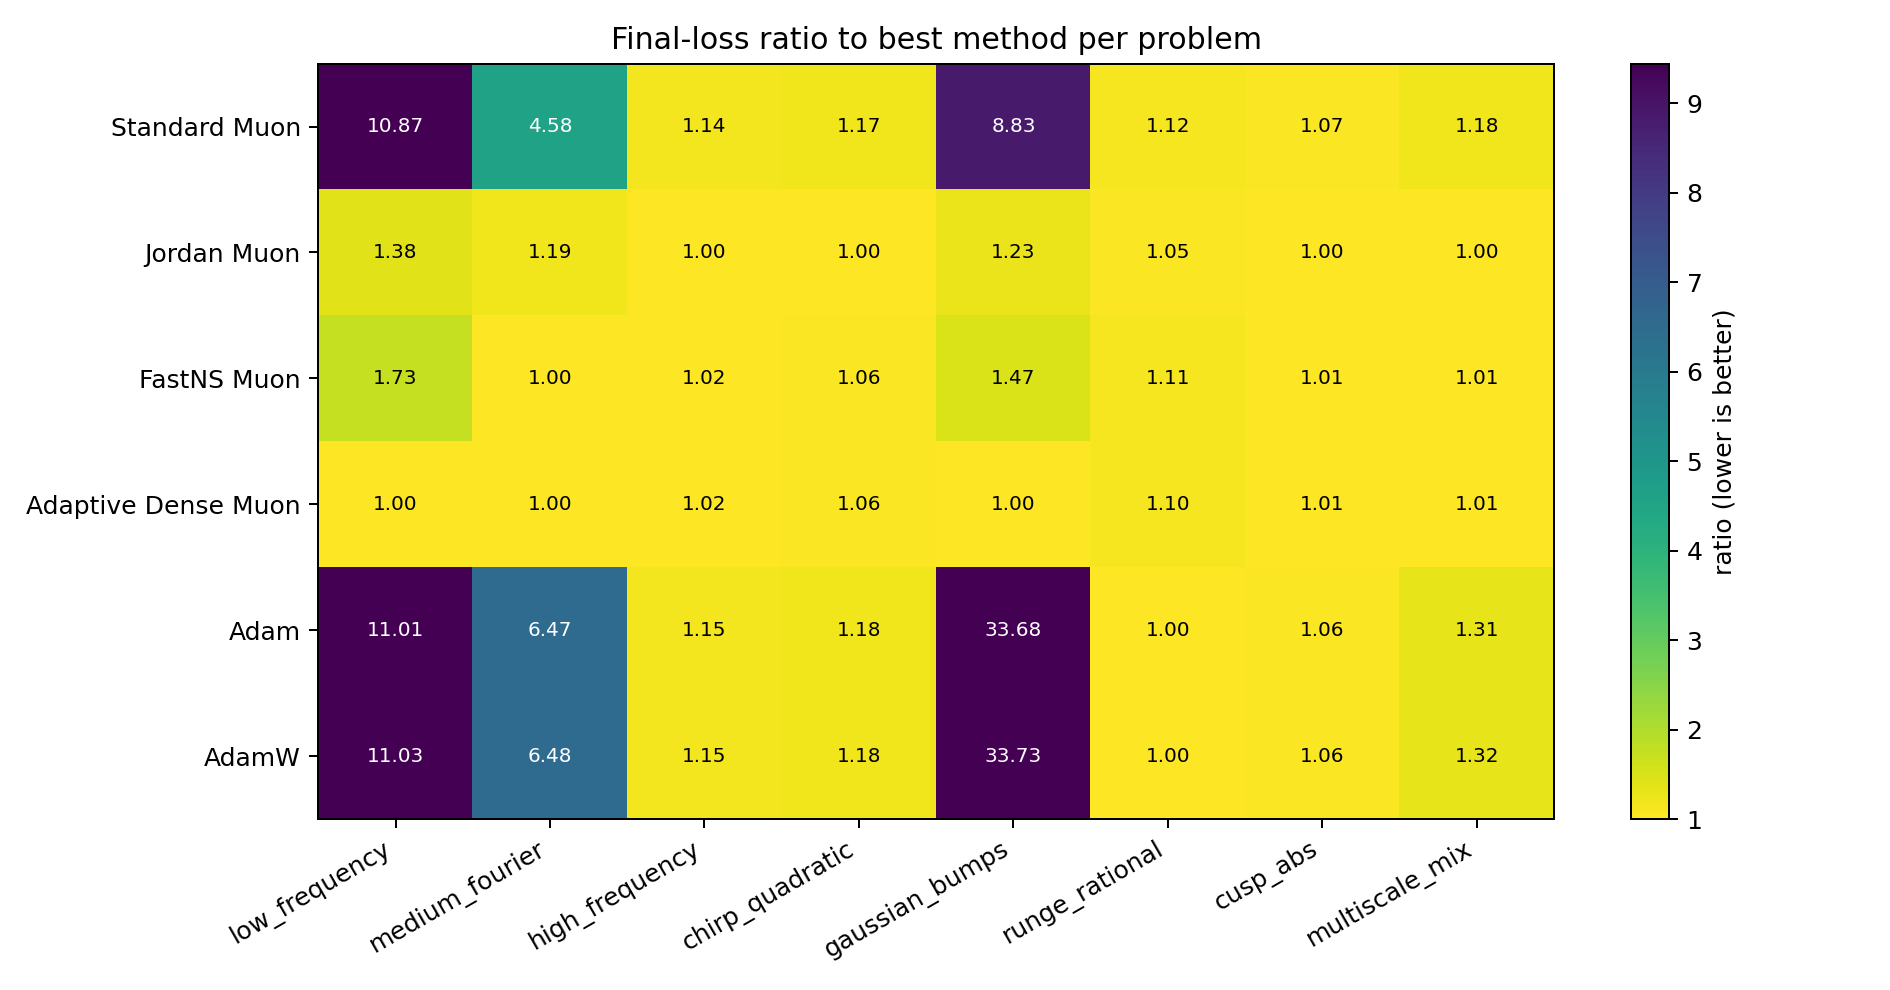
\includegraphics[width=0.95\linewidth]{../figures/adaptive_ns_suite/final_loss_ratio_heatmap.png}
\caption{Final-loss ratio to the best method on each problem. Lower is better.}
\end{figure}

\subsection{Aggregate Summary}

\begin{table}[H]
\centering
\begin{tabular}{lrrrrr}
\toprule
Method & Final ratio & Min ratio & Wins & Mean spikes & Final $a$ \\
\midrule
Standard Muon & 2.317 & 2.636 & 0 & 0.00 & 1.50 \\
Jordan Muon & 1.099 & 1.170 & 4 & 0.49 & 3.44 \\
FastNS Muon & 1.152 & 1.014 & 1 & 16.17 & 3.87 \\
Adaptive Dense Muon & 1.024 & 1.015 & 3 & 12.09 & 3.82 \\
Adam & 2.862 & 3.248 & 1 & 0.00 & -- \\
AdamW & 2.864 & 3.250 & 0 & 0.00 & -- \\
\bottomrule
\end{tabular}
\caption{Aggregate metrics. Ratios are geometric mean ratios to the best method on each problem.}
\label{tab:aggregate}
\end{table}

\subsection{Adaptive Trigger Timing}

\begin{table}[H]
\centering
\begin{tabular}{lrrrrrr}
\toprule
Problem & Mean $t_0$ & Std. & Triggered & Prev. spikes & Curr. spikes & Delta \\
\midrule
low\_frequency & 362.2 & 24.6 & 100\% & 0.1 & 2.0 & 1.9 \\
medium\_fourier & -- & -- & 0\% & 0.1 & 0.0 & -0.1 \\
high\_frequency & -- & -- & 0\% & 0.0 & 0.1 & 0.1 \\
chirp\_quadratic & -- & -- & 0\% & 0.0 & 0.0 & 0.0 \\
gaussian\_bumps & 418.4 & 38.6 & 95\% & 0.2 & 1.9 & 1.7 \\
runge\_rational & 419.0 & 80.5 & 15\% & 0.0 & 0.3 & 0.3 \\
cusp\_abs & -- & -- & 0\% & 0.0 & 0.0 & 0.0 \\
multiscale\_mix & 491.0 & 0.0 & 5\% & 0.0 & 0.2 & 0.2 \\
\bottomrule
\end{tabular}
\caption{Observed spike-frequency trigger timing for Adaptive Dense Muon. Spike counts are averages over the previous and current trigger windows at the final step of each initialization.}
\label{tab:adaptive-trigger}
\end{table}

\subsection{Loss Curves Across Initializations}

Each plot shows only method mean curves; faint shaded bands show one standard deviation across initializations.


\begin{figure}[H]
\centering
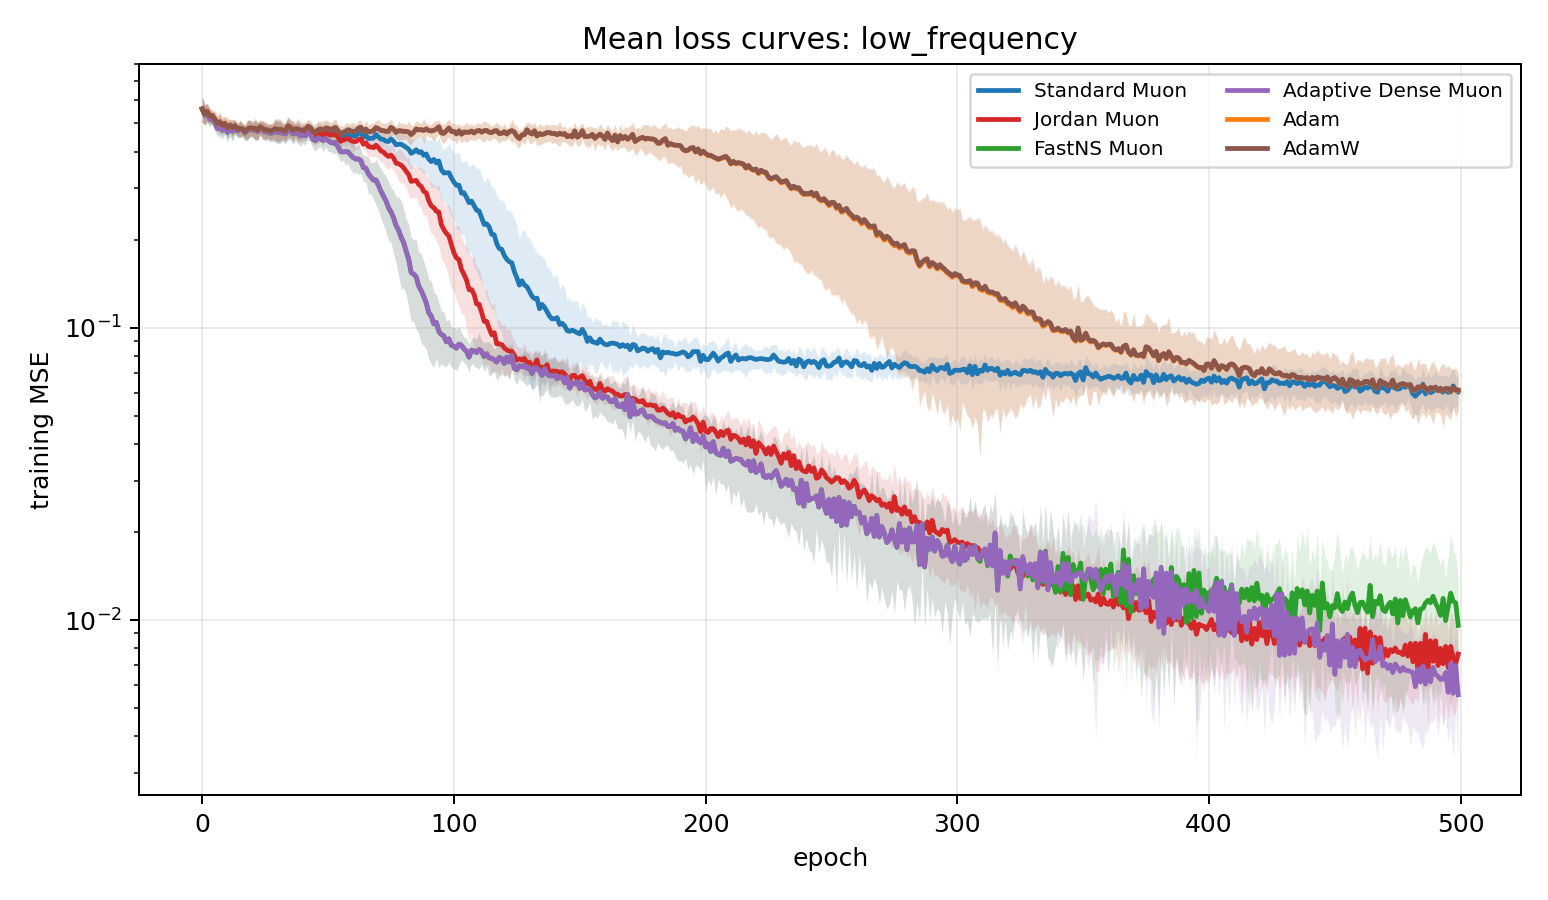
\includegraphics[width=0.92\linewidth]{../figures/adaptive_ns_suite/loss_curves/low_frequency_loss.png}
\caption{Mean loss curves over 20 initializations for \texttt{low\_frequency}. Shaded bands show one standard deviation across initializations.}
\end{figure}


\begin{figure}[H]
\centering
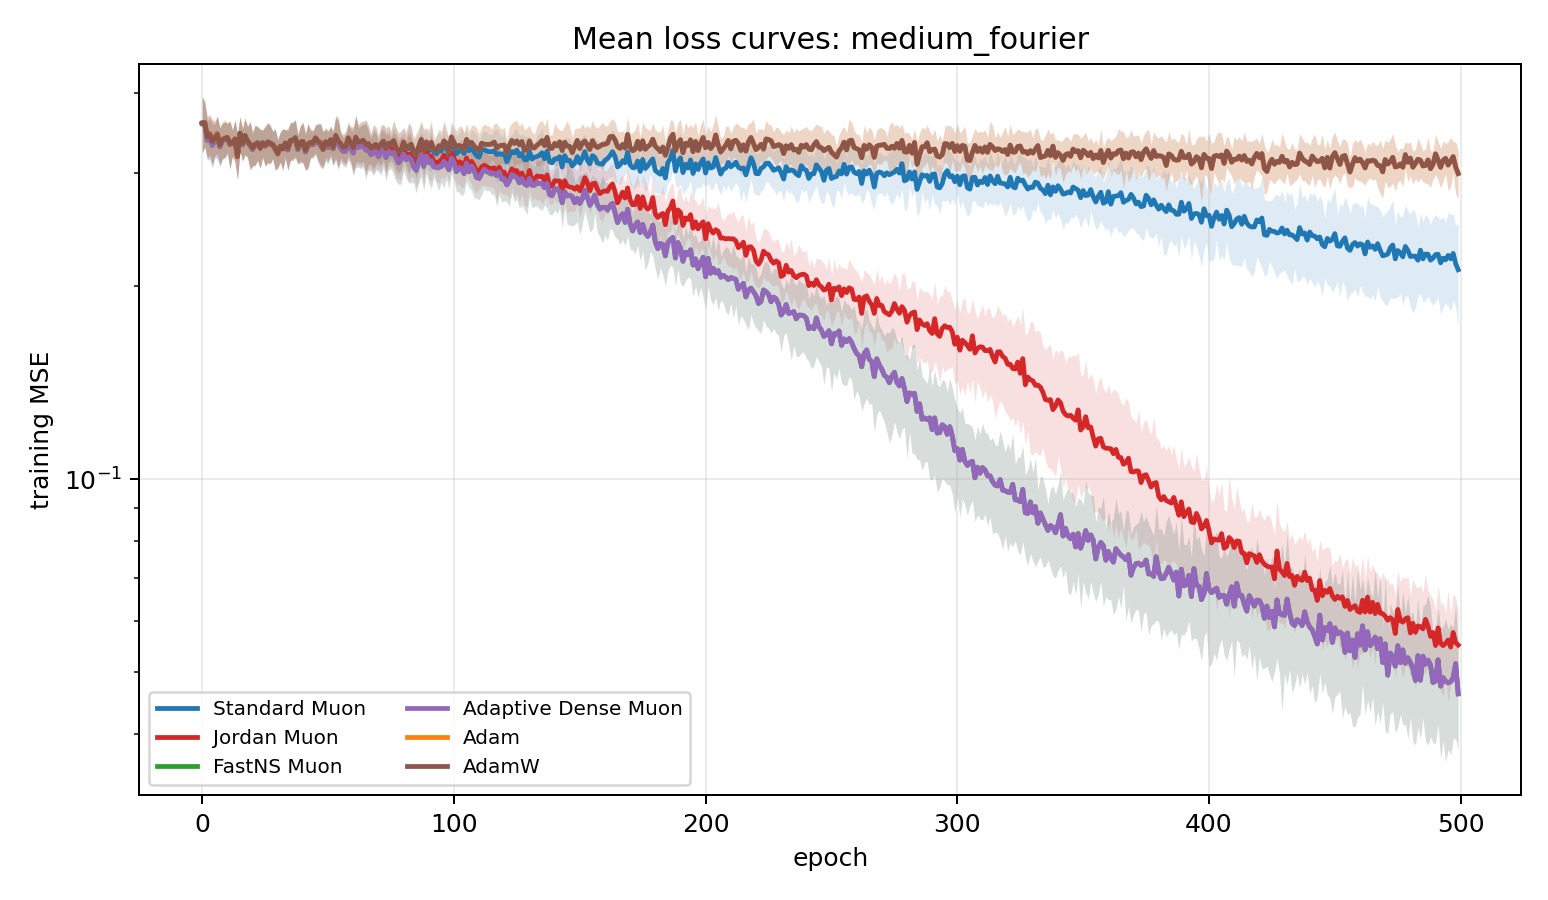
\includegraphics[width=0.92\linewidth]{../figures/adaptive_ns_suite/loss_curves/medium_fourier_loss.png}
\caption{Mean loss curves over 20 initializations for \texttt{medium\_fourier}. Shaded bands show one standard deviation across initializations.}
\end{figure}


\begin{figure}[H]
\centering
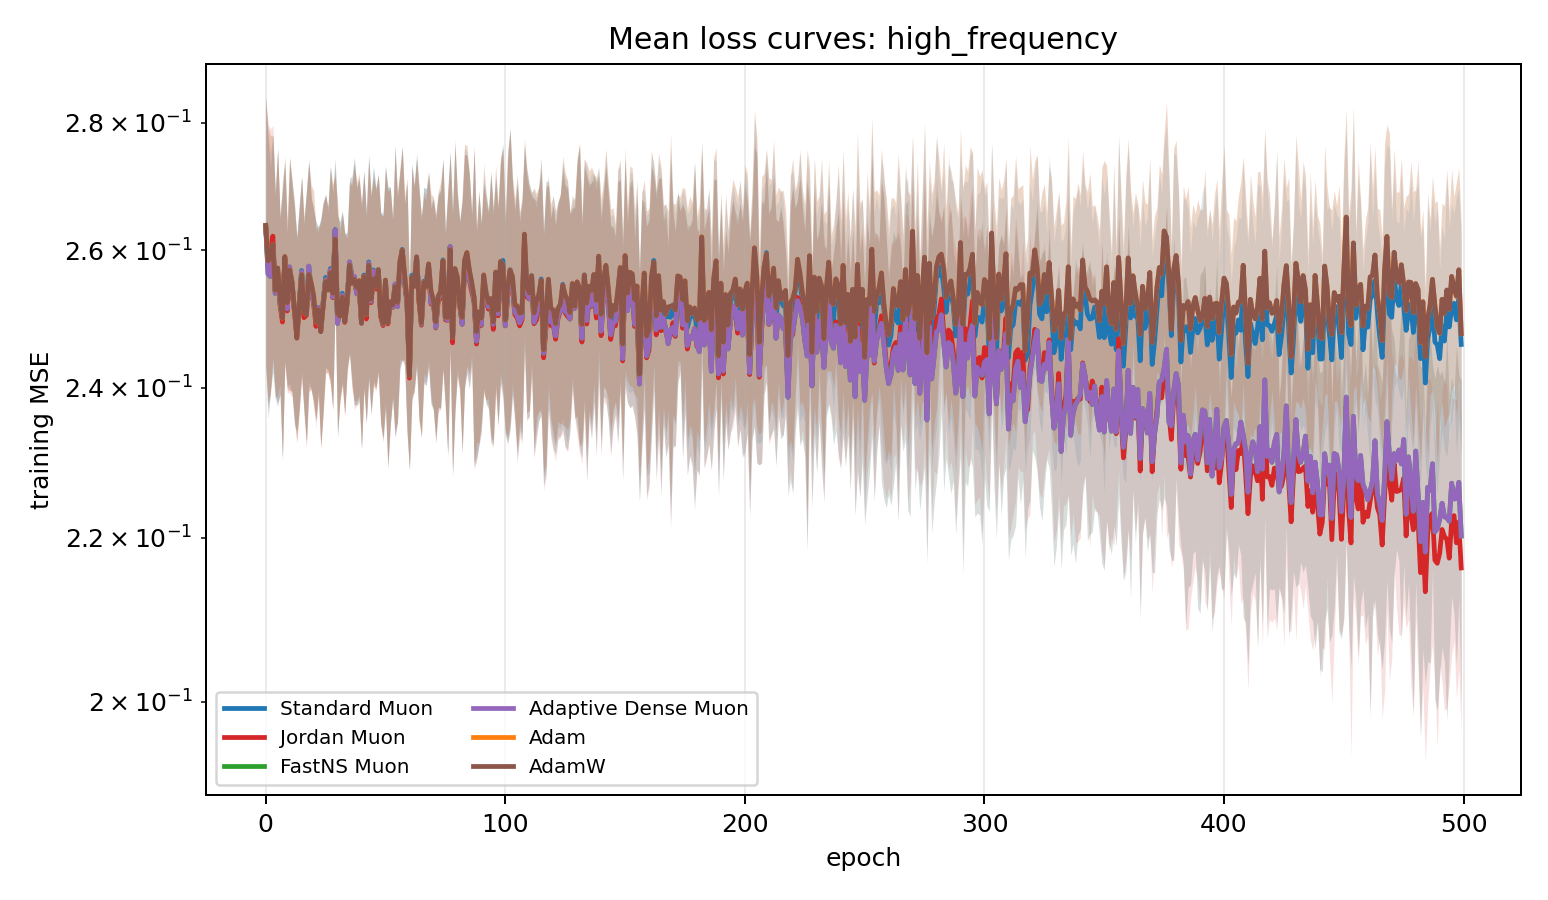
\includegraphics[width=0.92\linewidth]{../figures/adaptive_ns_suite/loss_curves/high_frequency_loss.png}
\caption{Mean loss curves over 20 initializations for \texttt{high\_frequency}. Shaded bands show one standard deviation across initializations.}
\end{figure}


\begin{figure}[H]
\centering
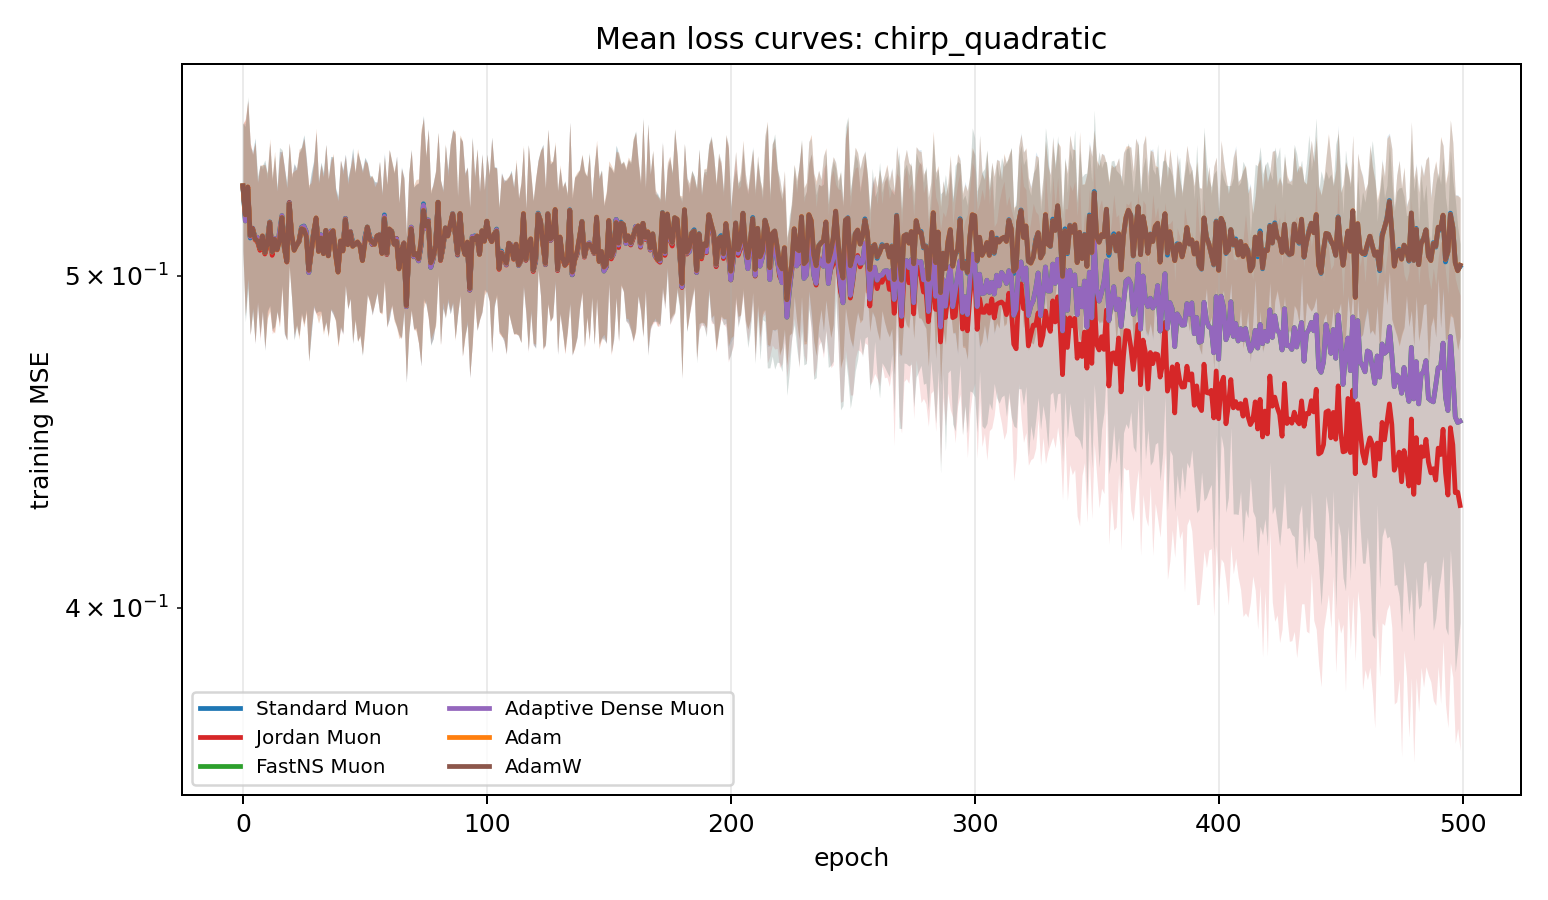
\includegraphics[width=0.92\linewidth]{../figures/adaptive_ns_suite/loss_curves/chirp_quadratic_loss.png}
\caption{Mean loss curves over 20 initializations for \texttt{chirp\_quadratic}. Shaded bands show one standard deviation across initializations.}
\end{figure}


\begin{figure}[H]
\centering
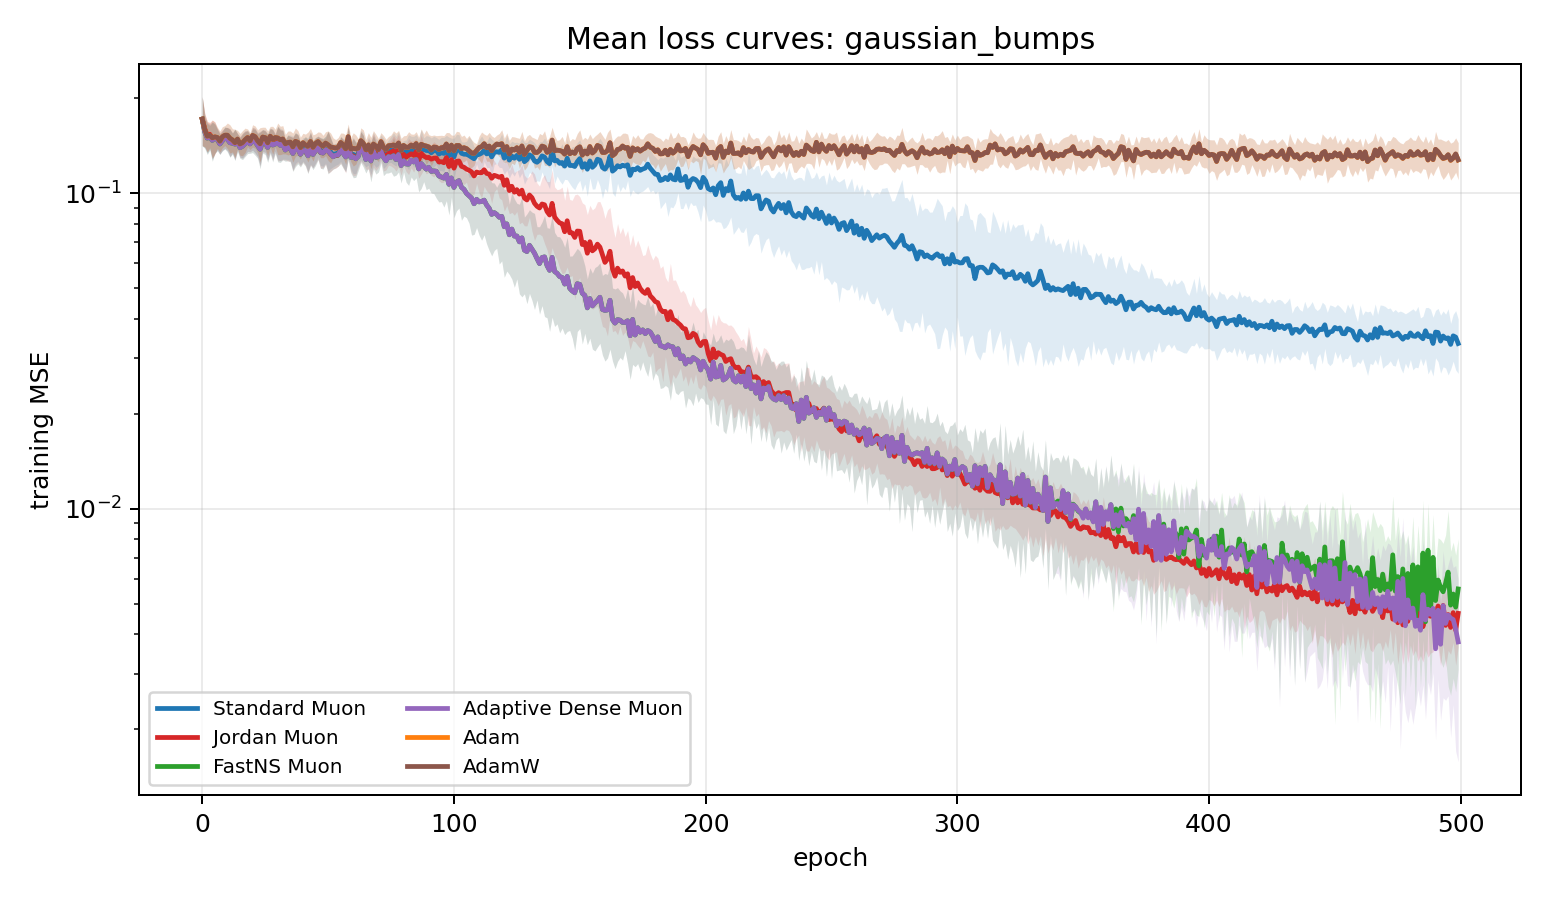
\includegraphics[width=0.92\linewidth]{../figures/adaptive_ns_suite/loss_curves/gaussian_bumps_loss.png}
\caption{Mean loss curves over 20 initializations for \texttt{gaussian\_bumps}. Shaded bands show one standard deviation across initializations.}
\end{figure}


\begin{figure}[H]
\centering
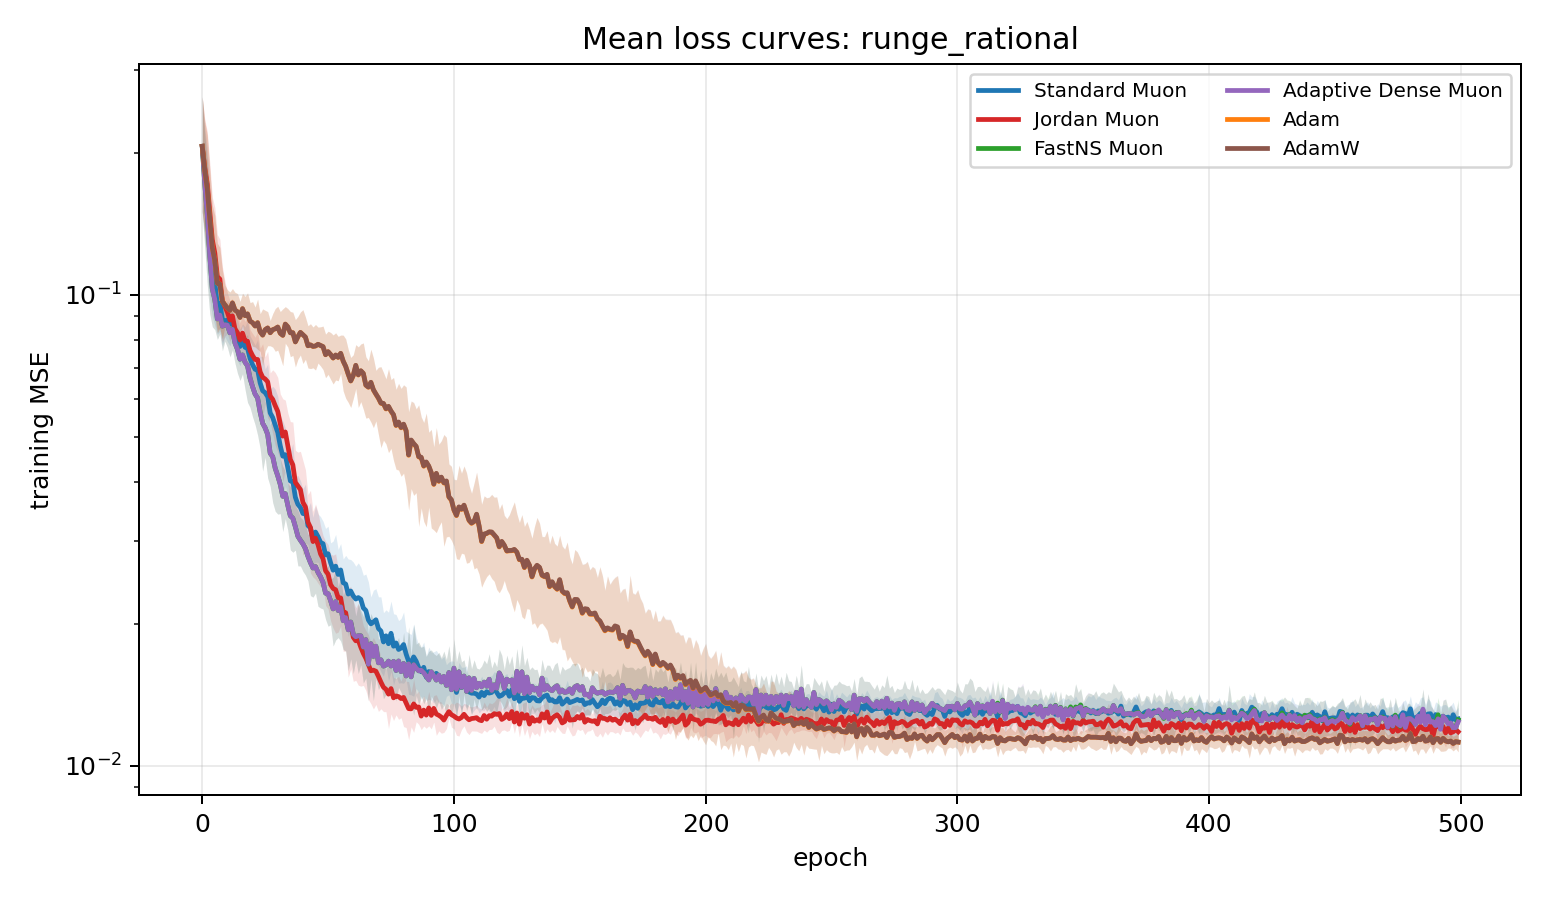
\includegraphics[width=0.92\linewidth]{../figures/adaptive_ns_suite/loss_curves/runge_rational_loss.png}
\caption{Mean loss curves over 20 initializations for \texttt{runge\_rational}. Shaded bands show one standard deviation across initializations.}
\end{figure}


\begin{figure}[H]
\centering
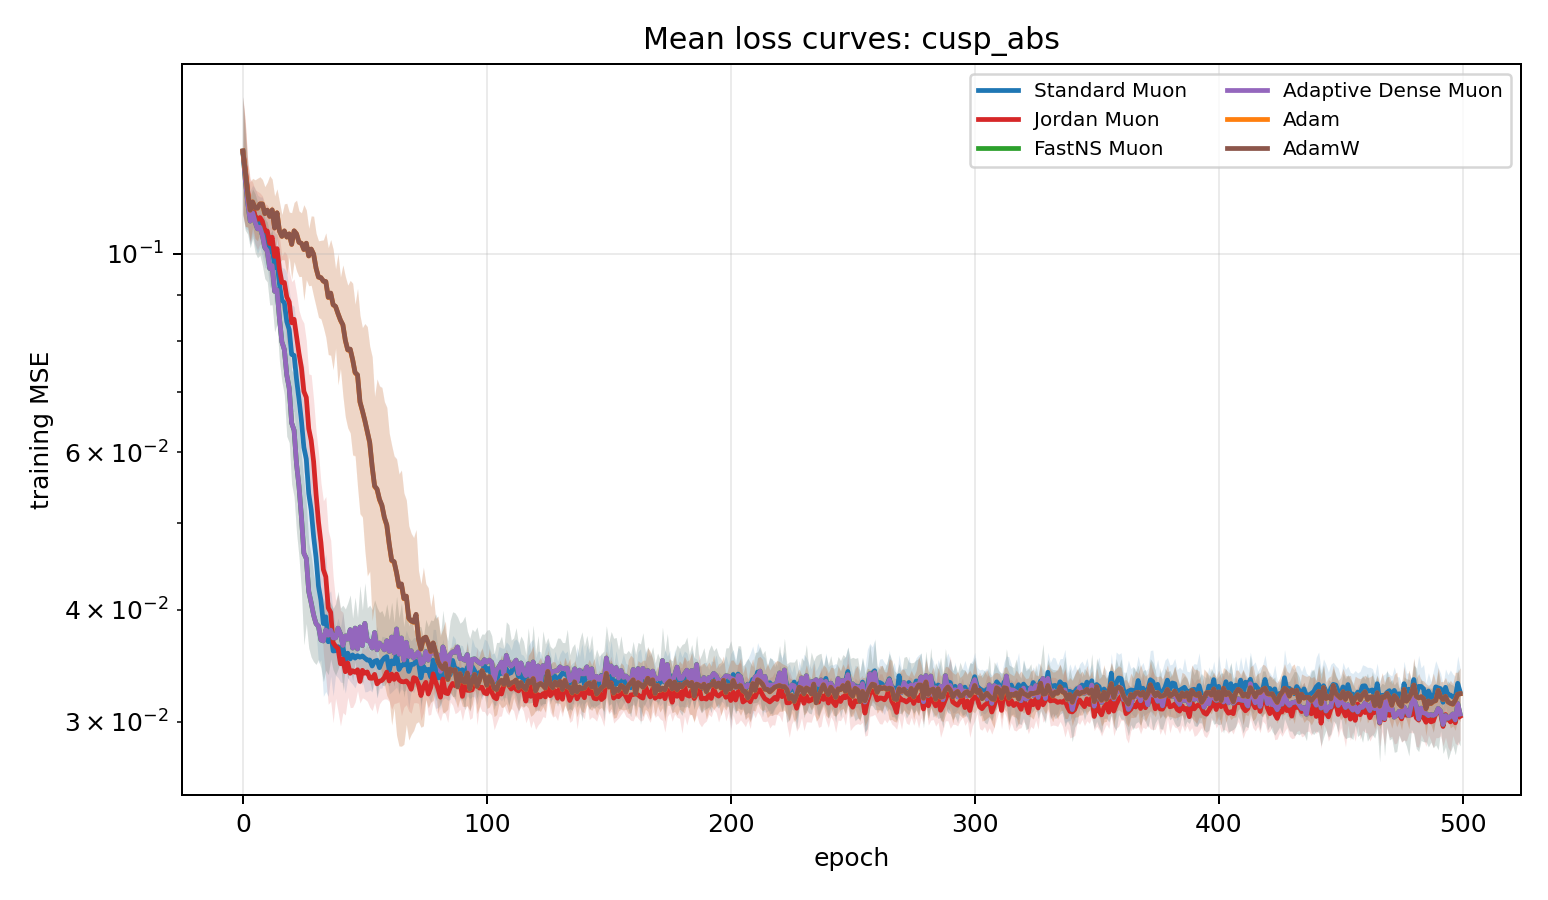
\includegraphics[width=0.92\linewidth]{../figures/adaptive_ns_suite/loss_curves/cusp_abs_loss.png}
\caption{Mean loss curves over 20 initializations for \texttt{cusp\_abs}. Shaded bands show one standard deviation across initializations.}
\end{figure}


\begin{figure}[H]
\centering
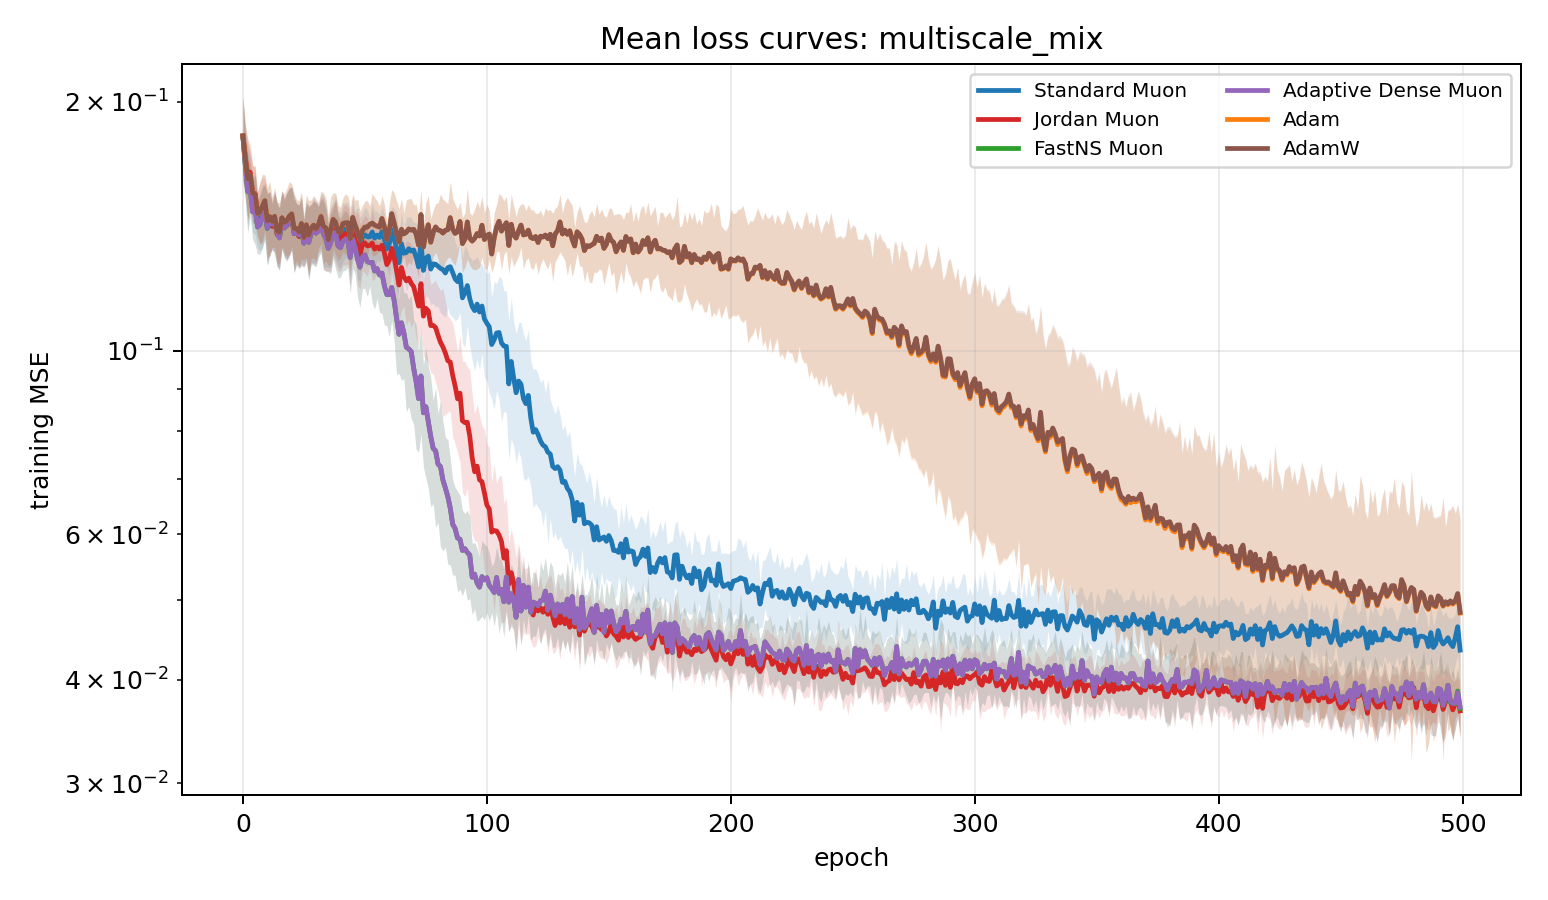
\includegraphics[width=0.92\linewidth]{../figures/adaptive_ns_suite/loss_curves/multiscale_mix_loss.png}
\caption{Mean loss curves over 20 initializations for \texttt{multiscale\_mix}. Shaded bands show one standard deviation across initializations.}
\end{figure}



\section{Discussion}

The final-loss winners are distributed as follows: Jordan Muon (4), FastNS Muon (1), Adaptive Dense Muon (3), Adam (1). The per-problem
table above gives the individual winners and ratios, but the main pattern in the
loss curves is not simply final-loss dominance. FastNS, and the adaptive method
before it triggers, often provide faster early decay because the large initial
$a$ aggressively amplifies small singular modes. This early advantage is clearest
on the smoother or easier targets, while the harder oscillatory, chirp, cusp, and
multiscale cases show smaller or less reliable final-loss separation.

Adaptive Dense Muon currently uses a one-parameter FastNS-to-fallback table
schedule rather than the legacy loss-spike dense-table controller. The schedule
changes only the scalar target $a$; each step still uses a prepared table triple.
FastNS is the no-trigger fallback: the method starts at FastNS, and if the spike
trigger never fires, it remains exactly the fixed FastNS optimizer. In this run
that exact fallback behavior occurs on medium Fourier, high-frequency, chirp,
and cusp. It switches only when relative loss spikes become more frequent in the
current window than in the previous window. Its mean final $a$ is
3.82, and its mean spike count is 12.09,
compared with 16.17 for fixed FastNS. The reduced spike
count is useful, but this controller is not yet optimized: late triggers can have
little benefit, and difficult problems may need a different trigger, endpoint, or
schedule length. AdamW winning some targets remains useful evidence that
Adam/AdamW baselines should receive learning-rate sweeps before making broad
claims.

The current adaptive controller is deliberately simple. Better policies could use
stronger rollback rules, smoother table-key schedules, a smaller adaptive
ceiling, or per-iteration NS coefficient schedules.

\section{Reproducibility}

Regenerate all current experiment artifacts with:
\begin{verbatim}
python3 scripts/generate_all_experiments.py
\end{verbatim}

The main outputs are under \verb|results/adaptive_ns_suite/|,
\verb|figures/adaptive_ns_suite/|, and \verb|docs/|.

\end{document}
